\documentclass[a4paper,11pt]{scrartcl}

\usepackage[T1]{fontenc}
\usepackage[utf8]{inputenc}     % Zeichencodierung
\usepackage{graphicx}           % Graphiken
\usepackage[ngerman]{babel}     % Sprachpaket
\usepackage{setspace}           % Einstellungen für den Zeilenabstand
\usepackage{microtype}          % typografische Verbesserungen
\usepackage[colorlinks=false,pdfborder={0 0 0},bookmarksnumbered]{hyperref}
\usepackage{enumitem}
\usepackage[usenames,dvipsnames]{xcolor}
\usepackage{tabularx}

%%%%%%%%%%%%%%%%%%%%%%%%%%%%%%%
\newcommand{\enum}[1]{\begin{enumerate}[label=(\arabic*)]#1\end{enumerate}}
\newcommand{\art}[2]{\subsection*{#1} \enum{#2}}
\newcommand{\quot}[1]{\glqq #1\grqq}

\newcommand{\new}[1]{\textcolor{red}{#1}}

\newcounter{art}
\setcounter{art}{1}

\newcommand{\entry}[4]{#1 & #2 & #3 & #4\\}
\newcommand{\event}[4]{\item #1:\\1. #2\\2. #3\\3. #4}
%%%%%%%%%%%%%%%%%%%%%%%%%%%%%%%

\title{\Huge{Bierpongregelwerk}}
\author{Dominik, Felix, Leonhard, Lea, Marcel, Markus, Michael, Millane, \\Moritz G., Moritz W., Mukhtar, Sebbi, Sophie, Tim}
\date{\small{\today}}

\begin{document}
 
\maketitle
\vspace*{-1cm}
\center{\small{Version 1.4.1}}
\vspace*{2.5cm}
\begin{figure}[ht]
    \centering
    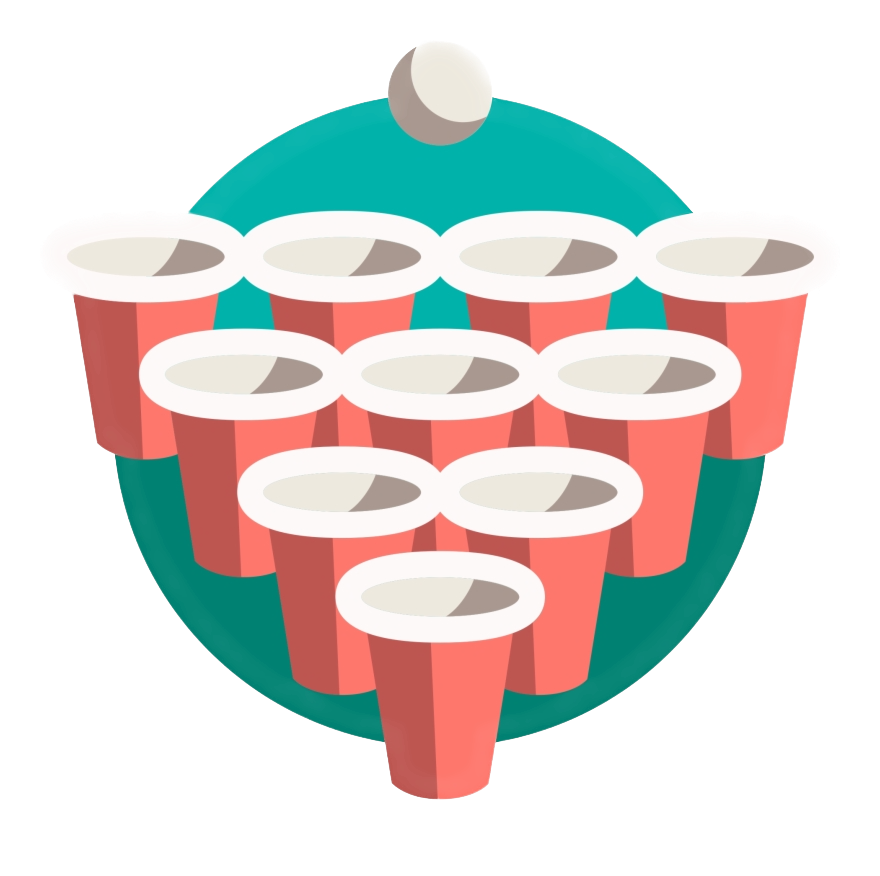
\includegraphics[width=0.5\textwidth]{images/title.png}
\end{figure}

\newpage

\section{Allgemeines}
    \art{Art \theart}{
        \item
            Wenn ein Becher getroffen wird, müssen alle Teammitglieder die vor Spielbeginn festgelegte Menge trinken.
    }
    \stepcounter{art}

    \art{Art \theart}{
        \item
            Es darf erst getrunken werden, wenn alle Würfe des gegnerischen Teams abgeschlossen sind.
        \item
            Wenn ein Teammitglied vergisst, vor der nächsten Runde zu trinken, darf das gegnerische Team eine angemessene Strafe für das gesamte Team festlegen. Eine Shotrunde wird empfohlen.
        \item
            Wenn sich das Spiel in der Endphase befindet und es sich um einen Konterwurf handelt, darf erst getrunken werden, wenn der Konterwurf nicht erfolgreich war.
    }
    \stepcounter{art}

    \art{Art \theart}{
        \item
            Bei jedem Specialwurf wird der Specialbecher immer entfernt.
        \item
            Bei Specialwürfen, bei denen mehr als nur der getroffene Becher entfernt wird, werden zuerst angrenzende Becher entfernt. Erst danach dürfen Becher entfernt werden, die nicht direkt an den Specialbecher angrenzen.
        \item
            Die zusätzlich zu entfernenden Becher dürfen vom Team ausgewählt werden, dem sie gehören.
    }
    \stepcounter{art}

    \art{Art \theart}{
        \item
            Im Falle eines Einzelspiels ist nicht erlaubt, dass ein Mitspieler beide Bälle gleichzeitig wirft.
        \item
            Im Falle eines Teamspiels ist erlaubt, dass ein/beide Mitspieler beide Bälle gleichzeitig wirft/werfen.
    }
    \stepcounter{art}

    \art{Art \theart}{
        \item
            Ein Spieler kann das andere Team auffordern, die Becher zu richten. Das gegnerische Team muss dieser Aufforderung nachkommen und die Becher richten.
        \item
            Das gegnerische Team darf die Becher nicht ohne Erlaubnis des anderen Teams richten.
    }
    \stepcounter{art}

    \art{Art \theart}{
        \item
            Ein Spieler kann das andere Team auffordern, den Ball aus einem Becher zu entfernen, wenn er darin ist. Das gegnerische Team darf dies auch ohne Aufforderung tun.
    }
    \stepcounter{art}

    \art{Art \theart}{
        \item
            Während das gegnerische Team die vor Spielbeginn festgelegte Menge trinkt, darf nicht geworfen werden.
        \item
            Wenn das gegnerische Team trotzdem trinkt, obwohl es nicht trinken muss, oder sich selbst durch andere Aktivitäten ablenkt, darf geworfen werden.
    }
    \stepcounter{art}

\section{Spielbeginn}
    \art{Art \theart}{
        \item
            Um die Spielreihenfolge und -seite festzulegen, erhält jeweils ein Spieler pro Seite einen Ball. Beide Spieler müssen nun gleichzeitig versuchen, einen Becher des gegnerischen Teams zu treffen.
        \item
            Beim Werfen müssen sich beide Spieler in die Augen schauen.
        \item
            Das Team des Spielers, der zuerst trifft, darf entscheiden, welches Team beginnt. Das Team des Spielers, der nicht trifft, darf entscheiden, auf welcher Tischseite die Teams spielen.
        \item
            Wenn beide Spieler treffen, muss der Wurf von denselben Spielern wiederholt werden.
    }
    \stepcounter{art}

\section{Spielende}
    \art{Art \theart}{
        \item
            Das Spiel endet, sobald ein Team keine Becher mehr hat.
        \item
            Wenn das Spiel mit einem Timer gespielt wird, ist es ebenfalls beendet, sobald der Timer abgelaufen ist. Wenn das Spiel zu diesem Zeitpunkt unentschieden steht, gewinnt das Team, das als Nächstes einen gegnerischen Becher trifft. Es gibt keinen Konter.
    }
    \stepcounter{art}

    \art{Art \theart}{
        \item
            Wenn das erste Team den letzten Becher des zweiten Teams trifft, hat das zweite Team die Möglichkeit zum Kontern. Wenn der Konter erfolgreich ist, werden keine Becher entfernt und das erste Team ist erneut an der Reihe.
        \item
            Ein Konterversuch ist erfolgreich, wenn das zweite Team mit der gleichen Anzahl an Würfen die gleiche Anzahl an Bechern trifft, wie das erste Team zum Ausmachen benötigt hat.
        \item
            Wenn der letzte Wurf des ersten Teams ein Specialwurf war, muss das zweite Team mit dem gleichen Specialwurf kontern.
        \item
            Es gibt keine Begrenzung, wie oft gekontert werden kann.
    }
    \stepcounter{art}

\section{Spielregeln}
    \art{Art \theart}{
        \item
            Jedes Team hat in jeder Wurfrunde zwei Standardwürfe.
        \item
            Durch Specialwürfe kann die Anzahl der Würfe pro Wurfrunde erhöht werden.
        \item
            Wenn ein Team aus mehr als einem Spieler besteht, müssen immer zwei verschiedene Spieler werfen. Wenn ein Team aus drei oder mehr Spielern besteht, muss in jeder Wurfrunde ein anderes Spielerpaar werfen.
    }
    \stepcounter{art}

    \art{Art \theart\ - Ellenbogen}{
        \item
            Beim Wurf muss der Ellenbogen hinter der Tischkante bleiben.
        \item
            Bei der Millane-Technik, wenn eine Person seitlich vom Tisch steht, muss auch der Ellenbogen hinter der verlängerten Tischkante bleiben.
        \item
            Die Millane-Technik darf nur angewendet werden, wenn dadurch kein anderer Spieler behindert wird.
    }
    \stepcounter{art}

    \art{Art \theart\ - \quot{Balls Back}}{
        \item
            Wenn in einer Wurfrunde beide Würfe getroffen werden, werden die Bälle dem aktuellen Werferteam zurückgegeben und das Team darf erneut werfen.
        \item
            Bevor erneut geworfen wird, müssen die beiden getroffenen Becher entfernt werden.
    }
    \stepcounter{art}

    \art{Art \theart\ - Aufsetzer}{
        \item
            Wenn ein Becher mit einem Ball getroffen wird, der mindestens einmal aufgesetzt hat, zählt dieser Treffer als zwei Treffer.
        \item
            Sobald ein Ball mindestens einmal auf dem Tisch oder einem Gegenstand auf dem Tisch aufgesetzt hat, darf er abgewehrt werden.
        \item
            Ein Ball zählt als Aufsetzer, sobald er mindestens einmal auf dem Tisch oder einem Gegenstand auf dem Tisch aufgesetzt hat.
    }
    \stepcounter{art}

    \art{Art \theart\ - Roller}{
        \item
            Roller zählen als Aufsetzer.
        \item
            Ein Ball zählt als Roller, wenn er mindestens zwei Becher berührt hat.
        \item
            Ein Ball, der nur den Becherrand berührt, bevor er in einen Becher geht, zählt nicht als Roller.
    }
    \stepcounter{art}

    \art{Art \theart}{
        \item
            Wenn ein Teammitglied während des Spiels einen oder mehrere Becher des eigenen Teams umwirft, muss ein Becher entfernt werden.
        \item
            Der letzte Becher darf nicht durch Umschmeißen entfernt werden. Hier wird an die Fairness der Mitspieler appeliert.
    }
    \stepcounter{art}

    \art{Art \theart\ - \quot{Blasen/Fingern}}{
        \item
            Es ist nicht erlaubt, einen Ball, der noch nicht komplett im Becher ist, mit \quot{Blasen} oder \quot{Fingern} zu retten.
    }
    \stepcounter{art}

    \art{Art \theart\ - \quot{Dead Cup}}{
        \item
            Wenn am Ende einer Runde ein getroffener Becher stehen bleibt, zählt dieser Becher als \quot{Dead Cup}. Wenn das gegnerische Team in einer der nachfolgenden Runden diesen Becher trifft, hat das Team, das den \quot{Dead Cup} getroffen hat, sofort gewonnen.
        \item
            Wenn ein Mitglied des Teams mit dem \quot{Dead Cup} bemerkt, dass sie einen \quot{Dead Cup} haben, dürfen sie diesen Becher entfernen. Dies darf jedoch nicht innerhalb einer gegnerischen Wurfrunde geschehen.
    }
    \stepcounter{art}

    \art{Art \theart\ - \quot{Trickshot}}{
        \item
            Wenn ein Ball nach einem Wurf zurück auf die eigene Tischseite rollt, also über die Mitte des Tisches, darf das aktuelle Werferteam den Ball holen. Der Spieler, der den Ball geholt hat, darf einen \quot{Trickshot} machen. Dieser muss nach den regulären Würfen geworfen werden. Außerdem werden zuerst von regulären Bällen getroffene Becher entfernt.
        \item
            Ein Ball gilt nur als zurückgerollt, wenn er auf der eigenen Tischhälfte liegt. Wenn er wieder in die gegnerische Hälfte zurückrollt, darf der Ball nicht mehr geholt werden.
        \item
            Becher, die von einem \quot{Trickshot} getroffen wurden, müssen sofort entfernt werden.
        \item
            Wenn ein \quot{Trickshot}-Ball auf die eigene Tischhälfte zurückrollt, kann dieser ebenfalls geholt werden, und ein weiterer \quot{Trickshot} kann gemacht werden.
        \item
            Ein \quot{Trickshot} zählt nicht als \quot{Air Ball}, wenn er hinter der Tischkante gefangen wird.
    }
    \stepcounter{art}

    \art{Art \theart\ - \quot{Bombe}}{
        \item
            Wenn in einer Wurfrunde beide Würfe eines Teams den gleichen Becher treffen, müssen dieser Becher und zwei weitere Becher entfernt werden.
        \item
            Eine \quot{Bombe} führt sofort zur Ausführung der \quot{Balls Back}-Regel.
    }
    \stepcounter{art}

    \art{Art \theart\ - \quot{On Fire}}{
        \item
            Wenn ein Spieler zwei Bälle hintereinander trifft, darf er \quot{Heating Up} rufen. Wenn derselbe Spieler einen weiteren dritten Becher hintereinander trifft und \quot{On Fire} ruft, ist er \quot{On Fire}. Er darf so lange werfen, bis er nicht mehr trifft.
        \item
            \quot{Heating Up} und \quot{On Fire} müssen nicht in der gleichen Wurfrunde gerufen werden.
        \item
            Wenn \quot{Heating Up} oder \quot{On Fire} nicht gerufen wurde, kann der Spieler beim nächsten Treffer in Folge \quot{Heating Up} oder \quot{On Fire} rufen.
        \item
            Die \quot{On Fire}-Würfe werden sofort nach dem Ausruf ausgeführt.
        \item
            Aufsetzer und andere Specialwürfe zählen nur als ein Treffer.
    }
    \stepcounter{art}

    \art{Art \theart\ - \quot{Island}}{
        \item
            Wenn ein Becher allein steht, also keine Nachbarn hat, kann ein Spieler \quot{Island} auf diesen Becher rufen. Wenn der Spieler den genannten Becher trifft, müssen der getroffene Becher und ein weiterer Becher entfernt werden. Wenn der Spieler anstelle des \quot{Island}-Bechers einen anderen Becher trifft, zählt der Treffer nicht.
        \item
            Jeder Spieler darf im gesamten Spiel einmal \quot{Island} rufen.
    }
    \stepcounter{art}

    \art{Art \theart\ - \quot{Air Ball}}{
        \item
            Wenn ein \quot{Air Ball} hinter der Tischkante gefangen wird, darf der Fänger des Balls (solange er im gegnerischen Team ist) in der nächsten Wurfrunde einen Ball doppelt werfen.
        \item
            Ein Ball zählt als \quot{Air Ball}, wenn er keinen Gegenstand oder ähnliches berührt und hinter der Tischplatte gefangen wird.
        \item
            Bälle, die seitlich neben den Tisch geworfen werden oder dort gefangen werden, zählen nicht als \quot{Air Ball}.
    }
    \stepcounter{art}

\section{Specialwurfkombinationen}
    \begin{itemize}
        \item
            Bombe mit Aufsetzer $\rightarrow$ Bombenbecher + 2 weitere (Bombe) + 1 Becher je Aufsetzer
        \item
            Island mit Aufsetzer $\rightarrow$ Islandbecher + 1 weiterer (Island) + 1 Becher je Aufsetzer
        \item
            Bombe mit Island $\rightarrow$ Bomben-/ Islandbecher + 2 weitere (Bombe) + 1 weiterer (Island)
    \end{itemize}

\newpage

\section{Ergebnisse und Platzierungen}
    \subsection{Bewertung (Einzel- und Teamturniere)}
    1. Platz: 5 Punkte\\
    2. Platz: 3 Punkte\\
    3. Platz: 1 Punkt

    \subsection{Bestenliste (Team)}
        \begin{tabularx}{\textwidth}[h]{X|ccc}
            \hline\hline
            \textbf{Name} & \textbf{Punkte} & \textbf{Siege} & \textbf{Teilnahmen}\\
            \hline\hline
            \entry{Dominik}{5}{1}{1}
            \hline
            \entry{Tim}{5}{1}{2}
            \hline
            \entry{Michael}{5}{1}{2}
            \hline
            \entry{Leonhard}{5}{1}{2}
            \hline
            \entry{Moritz W.}{4}{0}{2}
            \hline
            \entry{Sophie}{3}{0}{1}
            \hline
            \entry{Mukhtar}{3}{0}{2}
            \hline
            \entry{Markus}{3}{0}{2}
            \hline
            \entry{Marcel}{1}{0}{2}
            \hline
            \entry{Felix}{1}{0}{2}
            \hline
            \entry{Lea}{1}{0}{2}
            \hline
            \entry{Millane}{0}{0}{1}
            \hline
            \entry{Sebbi}{0}{0}{1}
            \hline\hline
        \end{tabularx}
    
    \subsection{Bestenliste (Einzel)}
        \begin{tabularx}{\textwidth}[h]{X|ccc}
            \hline\hline
            \textbf{Name} & \textbf{Punkte} & \textbf{Siege} & \textbf{Teilnahmen}\\
            \hline\hline
            \entry{Moritz G.}{6}{0}{2}
            \hline
            \entry{Markus}{5}{1}{2}
            \hline
            \entry{Millane}{5}{1}{2}
            \hline
            \entry{Leonhard}{1}{0}{2}
            \hline
            \entry{Moritz W.}{1}{0}{2}
            \hline
            \entry{Mukhtar}{0}{0}{2}
            \hline
            \entry{Sophie}{0}{0}{1}
            \hline
            \entry{Lea}{0}{0}{1}
            \hline
            \entry{Marcel}{0}{0}{1}
            \hline
            \entry{Felix}{0}{0}{1}
            \hline\hline
        \end{tabularx}

    \subsection{Turniere und Platzierungen (Team und Einzel)}
        \begin{tabularx}{\textwidth}[h]{X|lll}
            \hline\hline
            \textbf{Datum} & \textbf{1.} & \textbf{2.} & \textbf{3.}\\
            \hline\hline
            \entry{28.01.23}{Millane}{Moritz G.}{Leonhard}
            \hline
            \entry{10.02.23}{Tim \& Michael}{Sophie \& Moritz W.}{Marcel \& Felix}
            \hline
            \entry{05.03.23}{Dominik \& Leonhard}{Markus \& Mukhtar}{Lea \& Moritz}
            \hline
            \entry{23.04.23}{Markus}{Moritz G.}{Moritz W.}
            \hline\hline
        \end{tabularx}
\end{document}
